%        File: main.tex
%     Created: Thu Apr 12  9:00 AM 2011 C
% Last Change: Thu Apr 12 10:00 AM 2011 C
%    Based on: prelimPres.tex by Katy Huff
%\documentclass[11pt,handout]{beamer}
\documentclass[9pt]{beamer}
\usetheme[white]{Wisconsin}
%\title[short title]{long title}
\title[NESD and Funding]{The NESD and Federal Funding for Nuclear Energy}
%\subtitle[short subtitle]{long subtitle}
\subtitle[Students]{How Students get Funded}
%\author[short name]{long name}
\author[M. Gidden]{Matthew J. Gidden}
%\date[short date]{long date}
\date[4.17.2012]{April 17, 2012}
%\institution[short name]{long name}
\institute[UW-Madison]{University of Wisconsin-Madison}
% Page numbers.
\setbeamertemplate{footline}[page number]
% Those icons  in the references are terrible looking.
\setbeamertemplate{bibliography item}[text]


\begin{document}
%%%%%%%%%%%%%%%%%%%%%%%%%%%%%%%%%%%%%%%%%%%%%%%%%%%%%%%%%%%%%
%% From uw-beamer Here's a handy bit of code to place at 
%% the beginning of your presentation (after \begin{document}):
\newcommand*{\alphabet}{ABCDEFGHIJKLMNOPQRSTUVWXYZabcdefghijklmnopqrstuvwxyz}
\newlength{\highlightheight}
\newlength{\highlightdepth}
\newlength{\highlightmargin}
\setlength{\highlightmargin}{2pt}
\settoheight{\highlightheight}{\alphabet}
\settodepth{\highlightdepth}{\alphabet}
\addtolength{\highlightheight}{\highlightmargin}
\addtolength{\highlightdepth}{\highlightmargin}
\addtolength{\highlightheight}{\highlightdepth}
\newcommand*{\Highlight}{\rlap{\textcolor{HighlightBackground}{\rule[-\highlightdepth]{\linewidth}{\highlightheight}}}}
%%%%%%%%%%%%%%%%%%%%%%%%%%%%%%%%%%%%%%%%%%%%%%%%%%%%%%%%%%%%%

%||||---------------
\frame{
\titlepage
}
%---------------||||


%||||---------------
\frame{
\frametitle{Outline}
\tableofcontents[]
}
%---------------||||


%---------------||||
\section{Introduction}
% Overview : .tex
% put a repository model into cyclus
% that is capable of distinguishing between disposal choices
% and fuel cycle choices
% but is still speedy. 

\begin{frame}[ctb!]
  \frametitle{Introduction : Purpose}
  Fuel cycle simulators are designed to answer policy-related questions
  regarding transitions from one equilibrium state to another.

  \vspace{0.2cm}

  \pause
  A simulator answers the following questions as a function of its 
  parameter space:
  \begin{itemize}
    \item how much material exists
    \item where does that material reside
    \item from/to where and when is material transported
    \item what kinds of facilities are needed
    \item when is each type of facility needed
  \end{itemize}
\end{frame}

\begin{frame}[ctb!]
  \frametitle{Introduction : Cyclus}
  Cyclus is designed to provide a common fuel cycle simulator 
  framework.

  In this vein, we wish to show similar capabilities to other 
  simulators, e.g. VISION.

  This discussion will provide 
\end{frame}

\begin{frame}[ctb!]
  \frametitle{Introduction : VISION}
  VISION has surfaced as the industry standard simulator. It is well
  represented in the literature and can model most aspects of the
  fuel cycle. \cite{yacout_vision_2006}
  \begin{itemize}
    \item continuous material flows
    \item fleet-based facility deployment
    \item some regional modeling capability
    \item input/output via Excel
    \item simulation engine via Powersim
  \end{itemize}
  However, Powersim has its limitations...
  \begin{itemize}
    \item variables as a function of software level... did you get the academic or professional version?
    \item it's (relatively) expensive
    \item it's third party software
  \end{itemize}
\end{frame}

\section{DOE Budget Breakdown}
%||||---------------
\begin{frame}[ctb!]
  \frametitle{Entire DOE Budget}
  \begin{figure}[htbp!]
    \begin{center}
      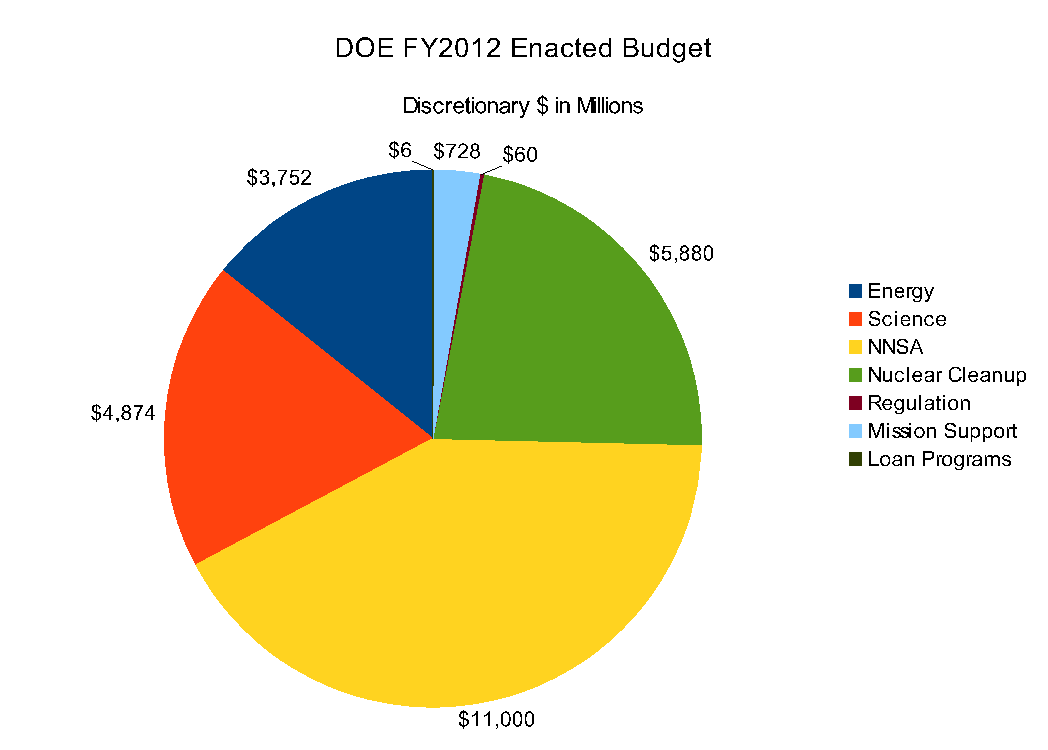
\includegraphics[height=6.5cm]{doe.eps}
    \caption{DOE Budget Breakdown by Office\cite{chu_2012}}
    \label{fig:doe}
    \end{center}
  \end{figure}
\end{frame}
%---------------||||

%||||---------------
\begin{frame}[ctb!]
  \frametitle{DOE Office of Energy Budget}
  \begin{figure}[htbp!]
    \begin{center}
      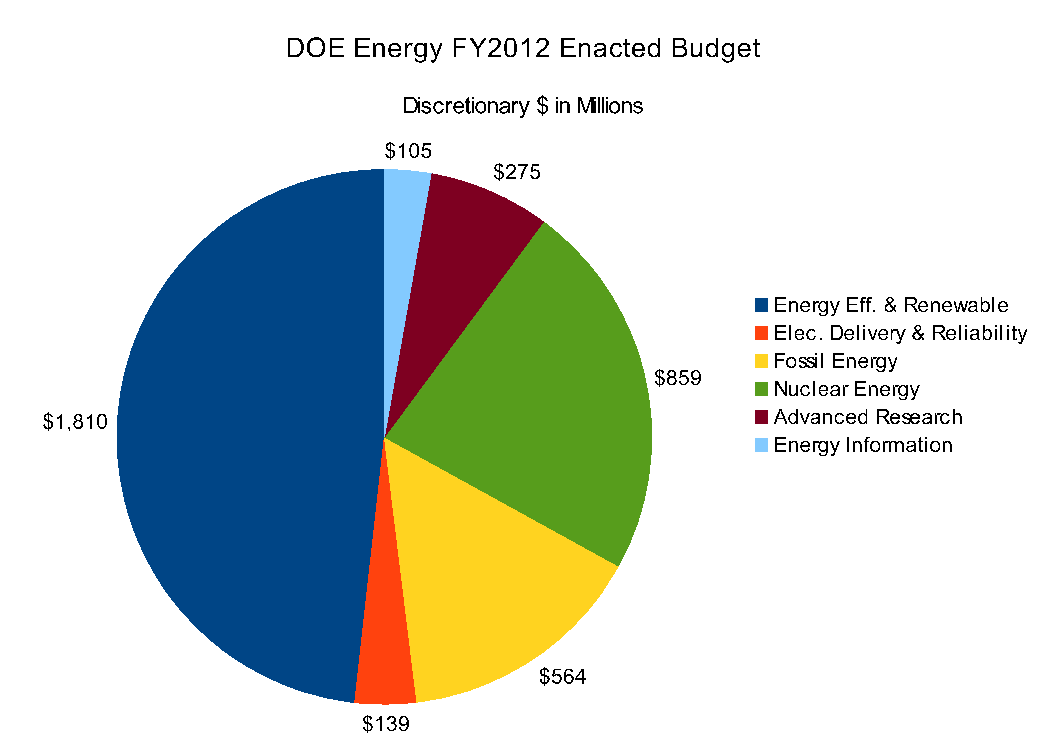
\includegraphics[height=6.5cm]{doe-e.eps}
    \caption{DOE-E Budget by Office\cite{chu_2012}}
    \label{fig:doe-e}
    \end{center}
  \end{figure}
\end{frame}
%---------------||||

%||||---------------
\begin{frame}[ctb!]
  \frametitle{DOE Office of Nuclear Energy Budget}
  \begin{figure}[htbp!]
    \begin{center}
      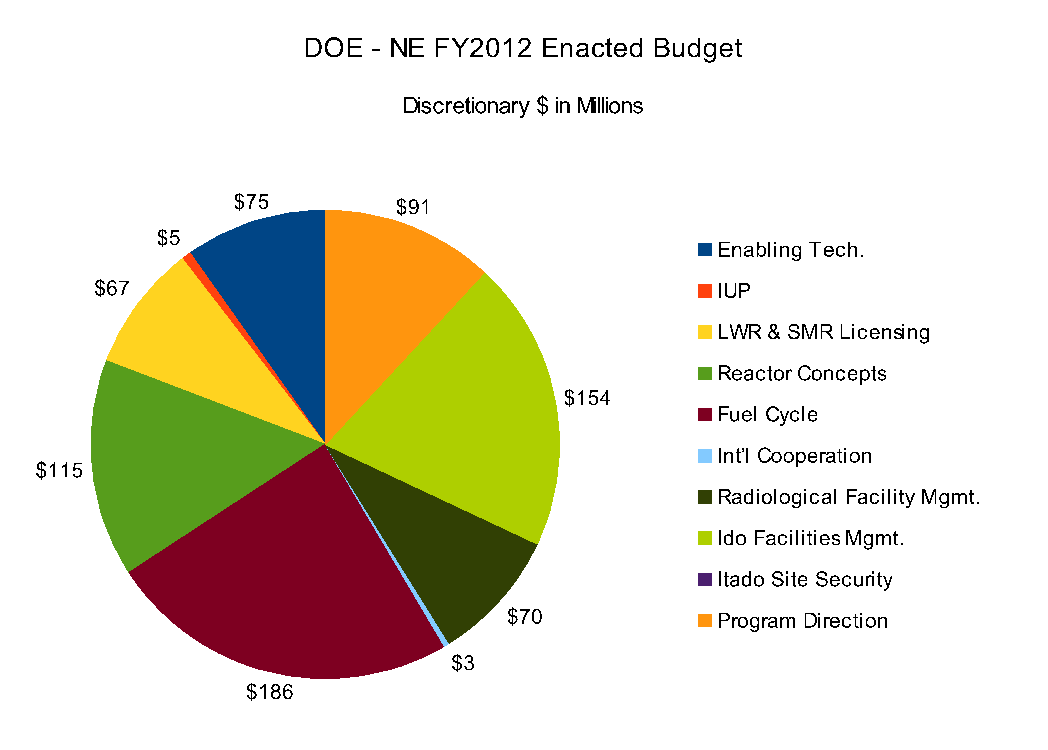
\includegraphics[height=6.5cm]{doe-ne.eps}
    \caption{DOE-NE Budget Breakdown by Office\cite{chu_2012}}
    \label{fig:doe-ne}
    \end{center}
  \end{figure}
\end{frame}
%---------------||||

\section{University Funding}
%||||---------------
\begin{frame}[ctb!]
  \frametitle{University Programs: NEUP}
  The Nuclear Energy University Partnership ``consolidates [the DOE-NE's] 
  university support under one program.''
  \vspace{0.4cm}
  \pause
  
  The NEUP funding pool
  \begin{itemize}
    \item is \emph{up to} 20\% of the DOE-NE's R&D budget (~\$60M)
    \item for infrastructure upgrade and maintenence
    \item for mission-critical R&D
  \end{itemize}
  \vspace{0.3cm}
  \pause
  
  The NEUP \emph{administrates} but \emph{does not provide funding} for
  DOE-NE funded scholarships and fellowships.
\end{frame}
%---------------||||

%||||---------------
\begin{frame}[ctb!]
  \frametitle{University Programs: NEUP}
  The Nuclear Energy University Partnership ``consolidates [the DOE-NE's] 
  university support under one program.''
  \vspace{0.4cm}
  \pause
  
  The NEUP funding pool
  \begin{itemize}
    \item is \emph{up to} 20\% of the DOE-NE's R&D budget (~\$60M)
    \item for infrastructure upgrade and maintenence
    \item for mission-critical R&D
  \end{itemize}
  \vspace{0.3cm}
  \pause
  
  The NEUP \emph{administrates} but \emph{does not provide funding} for
  DOE-NE funded scholarships and fellowships.
\end{frame}
%---------------||||

\section{NESD's Role}
%||||---------------
\begin{frame}[ctb!]
  \frametitle{NESD's Role: In General}
  Every year NESD meets for around 4 days.
  \begin{itemize}
    \item Meet with administration and others
      \begin{itemize}
        \item DOE - Assistant Secretary Lyons
        \item NRC - Commissioner Magwood
        \item CBO
        \item NEI
      \end{itemize}
    \item Write a policy statement
    \item Meet with representatives
  \end{itemize}
\end{frame}
%---------------||||

%||||---------------
\begin{frame}[ctb!]
  \frametitle{NESD's Role: A Student Voice}
  We try to provide the student's perspective to law makers via
  a policy statement.
  \begin{figure}[htbp!]
    \begin{center}
      
\includegraphics[height=5.5cm]{exec.eps}
    \caption{NESD 2011 Executive Summary}
    \label{fig:exec}
    \end{center}
  \end{figure}
\end{frame}
%---------------||||

%||||---------------
\begin{frame}[ctb!]
  \frametitle{NESD's Role: This Year}
  We will again enter a climate where the administration has
  zeroed out much of IUP.
  \vspace{0.4cm}
  \pause
  
  From ANS President, Eric Loewen's testimony\cite{loewen_testimony_2012}:
  \begin{quote}
    We urge the Subcommittee to support the continuation of the 
    Integrated University Program. Specifically, we request that 
    the Subcommittee to restore the full \$15 million in funding 
    for the Nuclear Regulatory Commission's portion of the IUP
    program and the \$5 million FY12 appropriated level for DOE-NE. 
  \end{quote}
\end{frame}
%---------------||||

%---------------||||


%||||---------------
\begin{frame}%[allowframebreaks]
  \frametitle{References}
  \bibliographystyle{plain}
  \bibliography{main}
\end{frame}
%---------------||||


%---------------||||
%||||---------------
\begin{frame}[ctb!]
  \frametitle{The Budget Making Process: Steps}
  The budget making process is, to say the least, involved.
  \begin{enumerate}
    \item President makes a budget request
      \begin{itemize}
        \item formulated by OMB
        \item IUP generally not in it
      \end{itemize}
    \pause
    \item Congress makes a budget resolution (like a guideline)
    \pause
    \item Congressional committees make authorizations (policy)
      \begin{itemize}
        \item IUP language introduced in 2009
        \item \$450M over 10 years split between ONE, NRC, NNSA
      \end{itemize}
    \pause
    \item Appropriations committee appropriates (funds)
  \end{enumerate}
  \pause
  The budget is then voted on and sent to the President. 
  The end result can be:
  \begin{itemize}
    \item Appropriations Bills from Committees
    \item Omnibus Bill (bring on the pork)
    \item Continuing Resolution
      \begin{itemize}
        \item occurs if no bill is signed into law by the end of 
          the fiscal year
        \item keeps funding at the same level as previous
        \item all of FY11 was a continuing resolution 
      \end{itemize}
  \end{itemize}
\end{frame}
%---------------||||



\end{document}
